\subsection{Strong Interactions}
\label{sec:Intro_QCD}

\begin{figure}[htb]
  \begin{center}
    {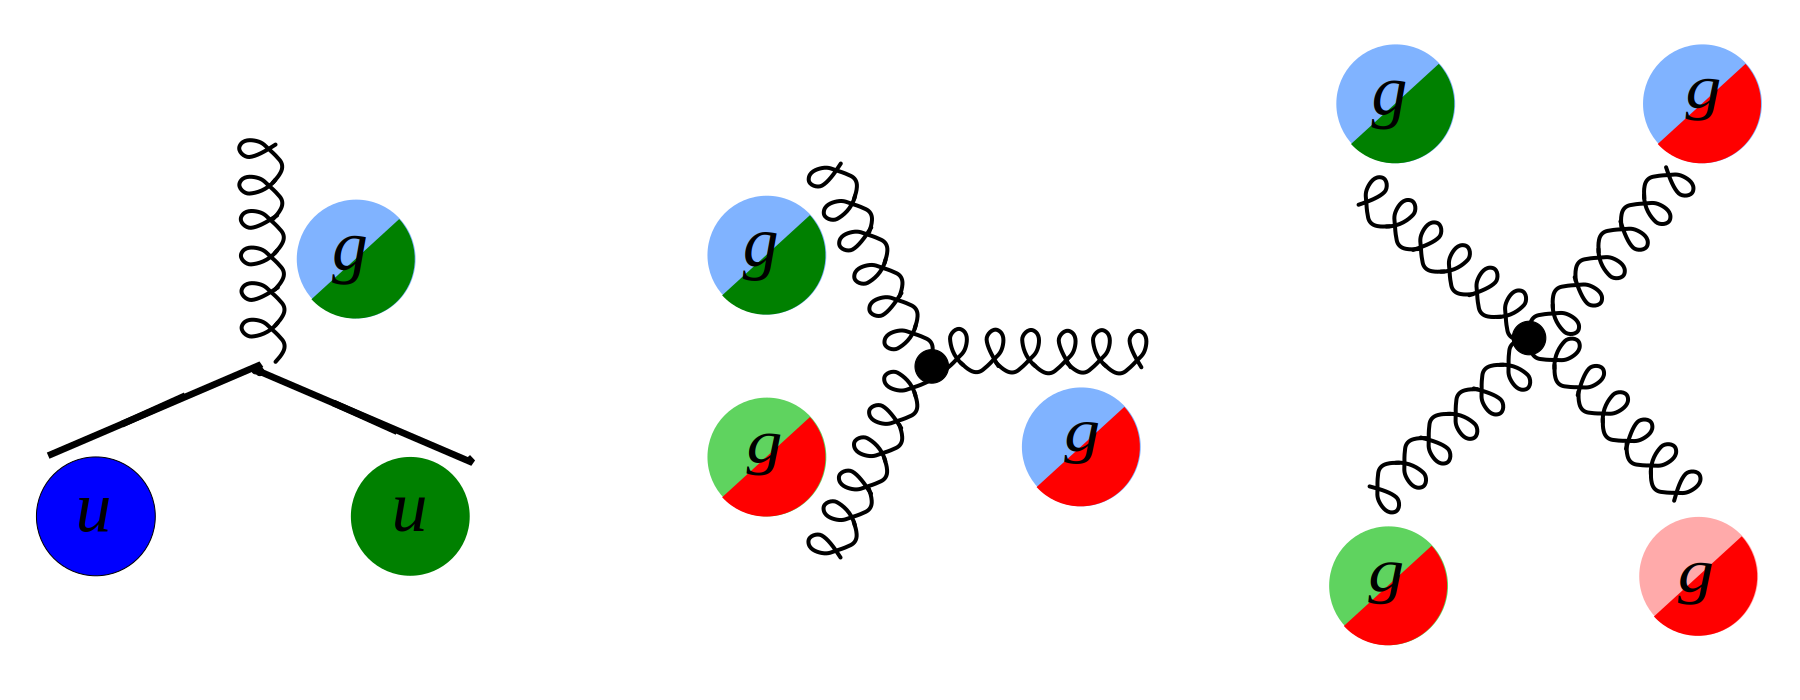
\includegraphics[width=0.90\textwidth]{../figs/Intro/feynmStrong.png}}
    \caption{Strong interations}
    \label{fig:feynmStrong}
  \end{center}
\end{figure}


The third fundamental force after the electromagnetic and weak ones is the strong force. The strong force is responsible for glueing protons and neutrons together in the nuclei as well as for forming protons and neutrons themselves. The strong interactions occur by exchanging gluons which are spin-one massless electrically neutral particles.  \\

The elementary strong processes are shown in Fig. \ref{fig:feynmStrong}. There are three elementary processes: qqg, ggg and gggg, all are involving particles with color charges. Thus, gluons couple to quarks and self-couple. Color charges must be conserved at each elementary process of the strong interaction. Because quarks can possess three colors, there are eight types of gluons to cover all possible color exchanges. \\

The coupling constant of the strong interaction depends on a distance between interacting particles: it becomes larger as the distance becomes larger. This property leads to two consequences specific to the strong force: the confinement and the asymptotic freedom.\\

The asymptotic freedom means that when quarks are very close to each other they almost do not interact with each other and therefore they are free. The confinement is the property of quarks to always stay in the color neutral combinations (hadrons), it forbids the existence of free quarks. A combination becomes colorly neutral when there is the same amount of color and anticolor or if there is the same amount of each of the three colors.  Thus, mesons are comprised of a quark and antiquarks with the opposite color charges, and baryons are comprised of three quarks: a red, a green and a blue one. Examples of baryons include such well-knowm particles as a proton and a neutron are baryons.\\

The strong interactions can be described by the quantum chromodynamics (QCD). QCD is a quantum field theory invariant under SU(3) color transformations. When the distance between quarks is small which corresponds to high energy, and thus the coupling constant $\alpha_s \ll 1$ is small, the perturbative approach can be used to compute observables.\\

The W$\gamma$ process being measured in this dissertation is not intended to test QCD, but a good understanding of QCD is essential for performing this measurement because the QCD corrections to the Feynman diagrams of the process are large and has to be taken into account in producing simulation. Possible QCD corrections include quark-gluon loops at any of three quark lines as well as exchanges of gluons between different quark lines. In addition, QCD describes the dynamics of quarks and gluons within colliding protons and predicts probabilities of one or another quark-antiquark pair to annihilate. Physics of proton-proton collisions is discussed in \ref{sec:Intro_ppCollisions}. \\
 
